\section{Overview}

This chapter will explain the general concept and architecture of the traffic light control system developed with this thesis. The traffic light control system will be built upon an existing traffic simulation. Which simulation is chosen will be discussed in a later section of the thesis and is not really relevant here, but this architecture will influence which traffic simulation will be chosen and what requirements it has to meet.

\begin{figure}[ht]
	\centering
  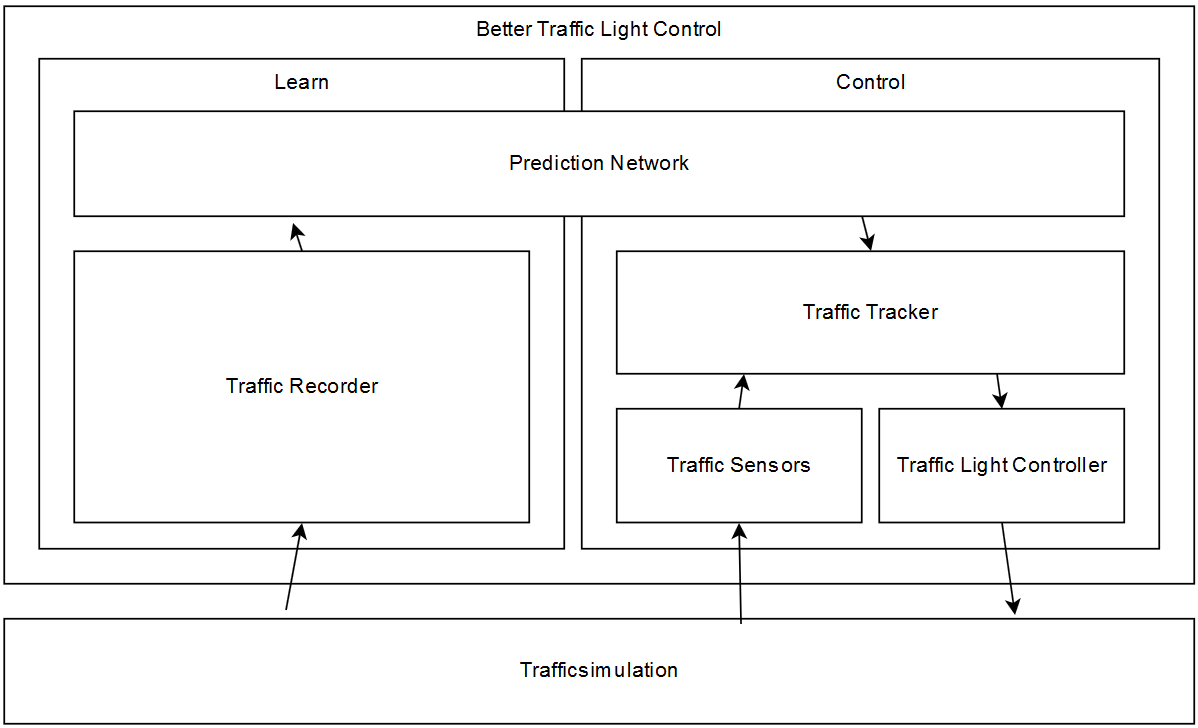
\includegraphics[width=16cm]{figures/architecture.png}
	\caption[Architecture of the Traffic Light Control System]{Architecture of the Traffic Light Control System \protect\footnotemark}
	\label{architecture}
\end{figure}

\footnotetext{own illustration}

The traffic light control system is separated into general areas, the learning part of the system and the controlling part. Either the system just observes a running traffic simulation and learns the patterns of the traffic or it observes the simulation through traffic sensors and controls the traffic lights according to the predictions fed by the traffic sensors. It is imaginable to let the system learn from a simulation and control it at the same time, but this is outside of the scope of this thesis. This could possibly improve the results and make it more practicable for a real world deployment.

== Why was that split done? ==

Spanning both the learning and the control part of the system is the prediction network. It is responsible for actually learning the traffic behavior and feeding predictions of the learned behavior back into a real simulation. For this task the prediction network will include an artificial neural network or multiple of them in some form, that is detailed in section \ref{predictionNetwork}. The prediction network will use reinforcement learning to learn the traffic patterns, meaning that there will not be labeled or unlabeled data sets collected beforehand, but the data sets will be collected on the fly from a running traffic simulation.

The traffic recorder will collect such data sets and feed them into the prediction network. It will observe the state of the traffic network and record the data that is compliant to the prediction networks input and output formats. With this component the creation of data sets is clearly separated from the prediction network. Thus it theoretically is possible to change the way data is fed to the prediction network easily. In a real world scenario it probably would be impossible to automatically record the data sets and it would be a huge benefit to easily swap out the learning input to some other method, which is totally possible with this architecture.

In the control part of the system the interaction with the traffic simulation occurs over traffic sensors that collect data and the traffic light controller that switches the states of the traffic lights. The different traffic sensors that are commonly used already are detailed in section \ref{trafficSensors}. Depending on the traffic simulation they are already part of the simulation or have to be simulated by observing the state of the simulation an extracting the relevant information. The traffic light controller has to switch the traffic lights depending on the input he gets from the traffic tracker and is further described in section \ref{trafficLightController}.

The final component of the architecture is the traffic tracker that keeps all other components together. Its task is to use the prediction network and the traffic sensors to create a picture of reality that has to closely match what is really happening. The traffic tracker can then make a statement about where cars should be in the system an the traffic light controller can then, based upon the traffic trackers data, make decisions how the traffic lights have to be optimally switched. The difficulties arising in this component are various. A traffic sensor could discover that a  prediction made by the prediction network is wrong. This has to be corrected somehow, but with a complex street network it may not be easy to detect where the failure came from. Furthermore traffic sensors may give very vague or heterogeneous data, making it hard to incorporate the data into the picture of reality.

== Maybe find a good figure / example to include here for the prediction sensor problem / maybe analogy with multilayer perceptrons ==

With this architecture it should be possible to experiment with different traffic sensors and traffic light controllers. This is a huge benefit, because experimentation will especially be important when trying to find the best setup of sensors and controller when later evaluating different possibilities to use the traffic light control system.

\section{Traffic Light Controller}
\label{trafficLightController}

== stress calculation ==

\section{Prediction Network}
\label{predictionNetwork}

=== Maybe a perceptron is enough for the prediction? ===

We tried the prediction network with an input for the amount of cars that want to pass, but this did introduce unnecessary complexity and the accuracy of the network went down

\section{Traffic Simulation Requirements}